% =====================================================================
%  THE SIGNAL — Newsletter of the Human-Technology Interaction Lab
%  K-12 Education in Physiological Computing  (Draft Issue, Fall 2026)
%  LaTeX source.  Compile with:  latexmk -pdf newsletter.tex
% =====================================================================
\documentclass[10pt,letterpaper]{article}

\usepackage[T1]{fontenc}
\usepackage[utf8]{inputenc}
\usepackage{newtxtext,newtxmath}        % Times-like editorial serif
\usepackage{microtype}
\usepackage[letterpaper,margin=0.68in,top=0.6in,bottom=0.72in]{geometry}
\usepackage{xcolor}
\usepackage{multicol}
\usepackage{enumitem}
\usepackage{booktabs}
\usepackage{tabularx}
\usepackage{tcolorbox}
\usepackage{tikz}
\usepackage{fancyhdr}
\usepackage{lastpage}
\usepackage{ragged2e}

\usetikzlibrary{positioning,arrows.meta,calc}
\tcbuselibrary{skins}

% ---------------- palette (single UA-crimson accent) ----------------
\definecolor{htilred}{HTML}{9E1B32}
\definecolor{htilgray}{HTML}{5C5C5C}
\definecolor{htilfaint}{HTML}{8A8A8A}
\definecolor{htiltint}{HTML}{F6F1F1}
\definecolor{htilrule}{HTML}{D9D9D9}
\definecolor{htilink}{HTML}{151515}

% ---------------- paragraph + list defaults ----------------
\setlength{\parindent}{0pt}
\setlength{\parskip}{4pt}
\raggedbottom
\setlist[itemize]{leftmargin=13pt,topsep=3pt,itemsep=2.5pt,parsep=0pt,label=\textcolor{htilred}{\textbullet}}

% ---------------- page furniture ----------------
\pagestyle{fancy}
\fancyhf{}
\renewcommand{\headrulewidth}{0pt}
\renewcommand{\footrulewidth}{0.4pt}
\fancyfoot[L]{\footnotesize\sffamily\color{htilfaint}\textls[110]{THE SIGNAL \textperiodcentered\ HTIL NEWSLETTER}}
\fancyfoot[C]{\footnotesize\sffamily\color{htilfaint}}
\fancyfoot[R]{\footnotesize\sffamily\color{htilfaint}\textls[110]{PAGE \thepage\ OF \pageref{LastPage}}}
\fancypagestyle{firstpage}{%
  \fancyhf{}\renewcommand{\headrulewidth}{0pt}\renewcommand{\footrulewidth}{0.4pt}%
  \fancyfoot[L]{\footnotesize\sffamily\color{htilfaint}\textls[110]{THE SIGNAL \textperiodcentered\ HTIL NEWSLETTER}}%
  \fancyfoot[R]{\footnotesize\sffamily\color{htilfaint}\textls[110]{PAGE \thepage\ OF \pageref{LastPage}}}}

% ---------------- reusable type ----------------
\newcommand{\eyebrow}[1]{{\sffamily\bfseries\color{htilred}\fontsize{7.4}{9}\selectfont\textls[150]{\MakeUppercase{#1}}}\par\vspace{1.5pt}}
\newcommand{\ruleaccent}{\noindent{\color{htilred}\rule{\linewidth}{2.5pt}}\par}
\newcommand{\hairline}{\noindent{\color{htilrule}\rule{\linewidth}{0.4pt}}\par}
\newcommand{\head}[1]{{\fontsize{22}{23.5}\selectfont\bfseries #1}\par\vspace{3pt}}
\newcommand{\headsm}[1]{{\fontsize{17.5}{19}\selectfont\bfseries #1}\par\vspace{3pt}}
\newcommand{\standfirst}[1]{{\fontsize{12}{15}\selectfont #1}\par\vspace{5pt}}
\newcommand{\deck}{\fontsize{11}{14}\selectfont}

% stat band: four (number, label) pairs
\newcommand{\statcell}[2]{{\color{htilred}\fontsize{18.5}{19}\selectfont\bfseries #1}\par\vspace{1pt}{\color{htilgray}\fontsize{7.2}{8.7}\selectfont #2}}
\newcommand{\statband}[8]{%
  \par\vspace{4pt}%
  \noindent{\color{htilink}\rule{\linewidth}{1.4pt}}\par\vspace{3pt}%
  \noindent\begin{tabularx}{\linewidth}{@{}X|X|X|X@{}}
    \statcell{#1}{#2} & \statcell{#3}{#4} & \statcell{#5}{#6} & \statcell{#7}{#8} \\
  \end{tabularx}\par\vspace{2pt}%
  \noindent{\color{htilrule}\rule{\linewidth}{0.4pt}}\par\vspace{2pt}}

% callout boxes
\tcbset{
  hbox/.style={enhanced, colback=htiltint, colframe=htilred, boxrule=0pt,
    toprule=2pt, bottomrule=0pt, leftrule=0pt, rightrule=0pt,
    arc=0pt, outer arc=0pt, sharp corners,
    left=8pt, right=8pt, top=6pt, bottom=7pt, fontupper=\small},
  obox/.style={enhanced, colback=white, colframe=htilrule, boxrule=0.5pt,
    arc=0pt, outer arc=0pt, sharp corners,
    left=8pt, right=8pt, top=6pt, bottom=7pt, fontupper=\small},
  boxhead/.style={fontupper=\small}
}
\newcommand{\boxhead}[1]{{\fontsize{10.5}{12}\selectfont\bfseries #1}\par\vspace{2pt}}

% tikz diagram styles
\tikzset{
  bx/.style={draw=htilrule, line width=0.5pt, fill=white, align=center,
             font=\scriptsize, inner sep=3pt, minimum height=11mm, text width=2.45cm},
  bxr/.style={bx, draw=htilred, line width=0.9pt, fill=htiltint},
  fl/.style={-{Latex[length=2.2mm,width=1.6mm]}, draw=htilred, line width=0.9pt},
  fld/.style={-{Latex[length=2.2mm,width=1.6mm]}, draw=htilfaint, line width=0.5pt, dashed}
}

% =====================================================================
\begin{document}
\thispagestyle{firstpage}
\setlength{\columnsep}{20pt}

% ============================== PAGE 1 ==============================
\ruleaccent
\vspace{6pt}

\noindent
\begin{minipage}[t]{0.70\linewidth}
  \eyebrow{Human--Technology Interaction Lab \textperiodcentered\ University of Alabama}
\end{minipage}%
\hfill
\begin{minipage}[t]{0.28\linewidth}\raggedleft
  \vspace{-2pt}{\sffamily\bfseries\color{htilred}\fontsize{7}{8}\selectfont\textls[120]{DRAFT FOR REVIEW}}
\end{minipage}

\vspace{2pt}
{\fontsize{40}{39}\selectfont\bfseries THE \textit{Signal}}\par
\vspace{2pt}
{\color{htilgray}\fontsize{8.6}{10.5}\selectfont K--12 Education in Physiological Computing \ \textbar\ \ Research from the Human--Technology Interaction Lab, Dept.\ of Computer Science, The University of Alabama}\par
\vspace{3pt}\hairline\vspace{4pt}

\noindent
\begin{minipage}[t]{0.70\linewidth}
  \eyebrow{Lead story}
  \head{Students Become the Technology}
  \standfirst{HTIL's K--12 program turns brainwaves and muscle signals into a hands-on route into computer science --- building the tools, curricula, and competitions that let students read, program, and control their own physiology.}
\end{minipage}%
\hfill
\begin{minipage}[t]{0.26\linewidth}\raggedleft\vspace{4pt}
  {\sffamily\color{htilfaint}\fontsize{7.4}{11}\selectfont\textls[80]{DRAFT ISSUE}\\ \textls[80]{FALL 2026}\\ \textls[80]{VOL.\ 1 \textperiodcentered\ NO.\ 1}\par}
  \vspace{3pt}
  {\sffamily\bfseries\color{htilred}\fontsize{7.4}{9}\selectfont\textls[80]{HTILUA.ORG}}
\end{minipage}

\vspace{2pt}
\begin{multicols}{2}
Physiological computing asks a simple but unfamiliar question: what if the computer's input device were your own body? In classrooms across Alabama, students place a sensor on their forearm or slip on an EEG headband and watch a live signal appear on screen --- a muscle's electrical activity, a brain's changing rhythms. Then they write the logic that turns that signal into action: a cursor that moves, a robot that walks, a drone that lifts off.

That real-time feedback loop is what makes the work stick. Students are not reading about technology from the outside; for the length of a lesson, they \emph{are} the sensor. Curiosity about ``can I control it?'' does the motivational work that worksheets usually have to do.

What started as a research question about brain--computer interfaces has grown into HTIL's largest education effort: a decade of classroom studies, a block-based programming environment used by students as young as 13, a national competition circuit, and an affordable hardware kit that can put a working biosignal station in a school for the price of a textbook. This issue is a snapshot of that work.
\end{multicols}

\statband
  {$\sim$\$7.5M}{Research funding supporting the lab's physiological computing and K--12 education programs}%
  {13}{Age of the youngest students building their own BCI applications with HTIL software}%
  {800+}{Media features and placements, including Forbes, The New York Times, and PBS NewsHour}%
  {Under \$25}{Target cost of a complete classroom biosignal station built on the lab's open EMG design}

\vspace{6pt}
\noindent
\begin{minipage}[t]{0.42\linewidth}
  \begin{tcolorbox}[obox]
    \eyebrow{In this issue}
    \vspace{-2pt}
    \begin{itemize}
      \item \textbf{NeuroBlock} --- block-based BCI for beginners
      \item \textbf{Curriculum} --- muscle signals in math class
      \item \textbf{Hardware} --- an EMG station for the price of a textbook
      \item \textbf{Teachers} --- the professional-development pipeline
      \item \textbf{Impact} --- publications, partners, and what's next
    \end{itemize}
  \end{tcolorbox}
\end{minipage}%
\hfill
\begin{minipage}[t]{0.55\linewidth}
  \eyebrow{Why it matters}
  {\small A single biosignal activity spans computer science, biology, data science, machine learning, signal processing, and engineering design at once --- and because every student's data is genuinely their own, there is no single right answer to copy.\par}
  \vspace{3pt}
  {\small Physiological computing education is a field HTIL has helped define, publishing the classroom evidence alongside the tools.\par}
\end{minipage}

\clearpage
% ============================== PAGE 2 ==============================
\eyebrow{Software \textperiodcentered\ NeuroBlock}
\headsm{Block-Based Brain--Computer Interfaces, Built for the First Try}
\standfirst{NeuroBlock lets a student assemble a working brain--computer interface the way they would assemble a Scratch project --- snapping logic, math, and hardware blocks together and running it against a live brain or muscle signal.}
\hairline
\vspace{4pt}

\noindent
\begin{minipage}[t]{0.615\linewidth}
  \begin{multicols}{2}
  NeuroBlock is a visual programming environment in the Scratch tradition, extended so that the signals feeding a student's program come from real sensors rather than a keyboard. Students drag blocks for logic, loops, math, and data processing, then connect them to blocks that read physiological data and drive connected hardware. No prior neuroscience background is required --- the environment does the signal handling so the student can focus on the program.

  It is deliberately hardware-agnostic at its core. Today NeuroBlock reads EEG from the \textbf{Muse 2} headband --- surfacing Delta, Theta, Alpha, Beta, and Gamma bands for students to reason about --- and muscle activity from the \textbf{OpenBCI Ganglion}. Output blocks control physical devices, including the \textbf{VEX AIM} robot and the \textbf{Tello} drone.

  The pedagogical bet is that a competition is the best curriculum. NeuroBlock's flagship event, the \textbf{Brain Drone Race}, asks competitors to out-focus one another: the electrical signals from their brains, not a joystick, steer the drone. It is a format that reads instantly to an audience and has carried the work into mainstream coverage.
  \end{multicols}
\end{minipage}%
\hfill
\begin{minipage}[t]{0.36\linewidth}
  \begin{tcolorbox}[hbox]
    \boxhead{NeuroBlock at a glance}
    \vspace{1pt}
    {\fontsize{8.2}{10}\selectfont
    \begin{tabularx}{\linewidth}{@{}>{\bfseries}p{1.65cm}>{\raggedright\arraybackslash}X@{}}
      Interface & Block-based, Scratch-like \\
      EEG input & Muse 2 --- Delta, Theta, Alpha, Beta, Gamma \\
      EMG input & OpenBCI Ganglion \\
      Outputs & VEX AIM robot \textperiodcentered\ Tello drone \textperiodcentered\ on-screen apps \\
      Youngest & Students as young as 13 \\
      Access & Open source; request at htilua.org/neuroblock \\
    \end{tabularx}\par}
  \end{tcolorbox}
  \vspace{6pt}
  \begin{tcolorbox}[obox]
    \boxhead{Selected publications}
    \vspace{1pt}
    \begin{itemize}
      \item \emph{Changing Minds: Exploring Brain--Computer Interface Experiences with High School Students}
      \item \emph{Brains and Blocks: Introducing Novice Programmers to Brain--Computer Interface Application Development}
      \item \emph{Brain--Computer Interface for Novice Programmers}
      \item \emph{NeuroBlock: A block-based programming approach to neurofeedback application development}
    \end{itemize}
  \end{tcolorbox}
\end{minipage}

\vspace{8pt}\hairline\vspace{6pt}
\eyebrow{From signal to program}
\vspace{3pt}
\begin{center}
\begin{tikzpicture}[node distance=5mm and 6mm]
  \node[bx]  (s)  {Sensor\\[1pt]\textcolor{htilgray}{EEG headband /}\\ \textcolor{htilgray}{EMG electrodes}};
  \node[bx,right=of s]  (c)  {Conditioning\\[1pt]\textcolor{htilgray}{Filter, band split,}\\ \textcolor{htilgray}{feature extraction}};
  \node[bxr,right=of c] (n)  {\textcolor{htilred}{NeuroBlock program}\\[1pt]\textcolor{htilgray}{Logic \textperiodcentered\ loops \textperiodcentered\ math \textperiodcentered}\\ \textcolor{htilgray}{thresholds students write}};
  \node[bx,right=of n]  (o)  {Output\\[1pt]\textcolor{htilgray}{Robot \textperiodcentered\ drone \textperiodcentered}\\ \textcolor{htilgray}{on-screen visual}};
  \node[bx,right=of o]  (f)  {Feedback\\[1pt]\textcolor{htilgray}{Student sees the}\\ \textcolor{htilgray}{loop close, adjusts}};
  \draw[fl] (s) -- (c);
  \draw[fl] (c) -- (n);
  \draw[fl] (n) -- (o);
  \draw[fl] (o) -- (f);
  \draw[fld] (f.south) -- ++(0,-3.5mm) -| (s.south);
\end{tikzpicture}
\end{center}
\vspace{-2pt}
{\color{htilfaint}\fontsize{7.5}{9}\selectfont\emph{The physiological computing pipeline students build against. HTIL's software handles the conditioning so beginners can start at the program.}}\par

\clearpage
% ============================== PAGE 3 ==============================
\eyebrow{Curriculum \textperiodcentered\ K--12}
\headsm{From Clenched Fists to Linear Functions}
\standfirst{The lab's curriculum work puts a biosignal in the middle of the math lesson. Students generate the data with their own bodies, then do the math on it --- counting, graphing, comparing fractions, fitting functions.}
\hairline
\vspace{4pt}

\begin{multicols}{2}
Physiological computing earns its classroom time by making abstract mathematics physical. A student who squeezes a sensor and watches the number rise is doing measurement before they have the word for it. A class that collects five peak values from five clenches and turns them into a bar graph is doing data analysis where every bar has a story. When the same data is used to compute a slope --- a peak value divided by the time it took to get there --- the function is something the student felt happen.

HTIL has mapped this approach across every grade band, from counting in kindergarten to vectors and conditional probability in high school, aligning each activity to state standards. The progression is deliberate: lower grades work with counting, pattern, and measurement; middle grades with data, ratios, and rate of change; upper grades with model fitting, classification, and inference.

\emph{``Every data point is personal. There is no single right answer for a classmate to copy.''}

\textbf{PhysioML} carries the idea into machine learning. It is a web-based environment where students apply ML concepts to real-time physiological data rather than to a pre-packaged dataset --- the same features-and-labels reasoning they meet in a textbook, but grounded in a signal their own body produced.

\textbf{PhysioBots} connects muscle signals directly to robot control, so the payoff of a well-chosen threshold is a machine that moves.
\end{multicols}

\vspace{6pt}\hairline\vspace{4pt}
\eyebrow{Sample activities across the grade bands}
\vspace{2pt}

{\fontsize{8.3}{10.2}\selectfont
\begin{tabularx}{\linewidth}{@{}>{\bfseries}p{1.55cm} p{3.0cm} X@{}}
\toprule
Grade band & Math focus & Physiological computing activity \\
\midrule
K--2 & Counting \& patterns & Each muscle clench is one count --- students count and compare their own totals. Squeeze-squeeze-rest becomes an AAB pattern they create and copy. \\
K--2 & Measurement & Compare a relaxed reading against a squeezed reading as a direct magnitude comparison of a live, self-generated biosignal. \\
3--5 & Data \& graphing & Collect peak values from repeated contractions and build a bar graph or line plot of their own muscle data --- real biological variability included. \\
3--5 & Fractions & Maximal contraction is the whole; students squeeze at one-half, one-quarter, and three-quarters of it, building fraction sense through proprioception and visual feedback together. \\
6--8 & Statistics & Take 100+ samples of a ``steady'' contraction and compute mean, median, and range --- then discuss biological noise as genuine variation, not error. \\
6--8 & Functions \& slope & Slope $=$ (peak $-$ baseline) $\div$ rise time. Students see the ramp and compute the rate at the same moment they feel it. \\
9--12 & Function families & Record fast-twitch, sustained-hold, and fatigue contractions, then compare fitted models by $R^2$ to ask which function actually describes a process. \\
9--12 & Conditional probability & A cursor-control game yields $P(\text{hit}\mid\text{intended up})$ and $P(\text{hit}\mid\text{intended down})$ --- students test whether their performance is meaningfully above chance. \\
9--12 & Vectors \& optimization & Four-channel signals become gesture vectors classified by distance; biofeedback turns ``satisfy two constraints at once'' into finding a feasible state in their own body. \\
\bottomrule
\end{tabularx}\par}

\vspace{6pt}
{\color{htilgray}\small Activities are written to sit alongside --- not replace --- the worksheets an Alabama classroom already uses. They are the lesson where the data is real.\par}

\clearpage
% ============================== PAGE 4 ==============================
\eyebrow{Hardware \textperiodcentered\ MioPod}
\headsm{A Classroom Biosignal Station for the Price of a Textbook}
\standfirst{Commercial EMG equipment runs from a few hundred to a few thousand dollars per unit --- a non-starter for most schools. The lab's open ESP32-based design targets a complete station for under \$25.}
\hairline
\vspace{4pt}

\noindent
\begin{minipage}[t]{0.615\linewidth}
  \begin{multicols}{2}
  The lab's affordable EMG platform --- \textbf{MioPod} --- starts from a hard constraint: the hardware has to be cheap enough that a teacher can kit out a classroom without a grant, and simple enough that a student can build and debug it. The design is built around an ESP32 module (roughly \$4 in parts at classroom quantities), which supplies the ADC, wireless radio, and processing headroom for a live biosignal dashboard without any accompanying computer beyond a laptop or Chromebook.

  On the analog side, the front end follows the classic instrumentation chain: a pre-amplifier, a band-pass filter tuned to the physiological EMG range of roughly 20--500~Hz, a notch filter to reject mains noise, and an envelope detector so a signal that swings positive and negative becomes a reading a student can plot. That chain is not hidden from learners --- building and testing it is part of the lesson, and students can see exactly why each stage exists.

  From there the ESP32 samples the signal, filters it digitally, and streams it wirelessly to a browser dashboard or to the same block-based environment students use elsewhere. The result is a station that covers signal acquisition, sensor design, filtering, wireless data, and visualization --- and that a school can afford to own thirty of.
  \end{multicols}
\end{minipage}%
\hfill
\begin{minipage}[t]{0.36\linewidth}
  \begin{tcolorbox}[hbox]
    \boxhead{Why build our own}
    \vspace{1pt}
    \begin{itemize}
      \item Commercial EMG sensors: \textbf{\$200--\$2,000+} per unit
      \item MioPod target BOM: \textbf{$\approx$\$4} in parts
      \item Complete station target: \textbf{under \$25}
      \item Open design --- students can inspect and rebuild every stage
      \item Wireless by default --- no tethered lab bench required
    \end{itemize}
  \end{tcolorbox}
  \vspace{6pt}
  \begin{tcolorbox}[hbox]
    \boxhead{Where it's been tested}
    \vspace{1pt}
    {\small The EMG platform has been validated in Alabama's Black Belt schools, and the lab is extending the model with interested partners in \textbf{Florida}, \textbf{Georgia}, \textbf{Illinois}, and the \textbf{D.C.--Maryland--Virginia} region.\par}
  \end{tcolorbox}
\end{minipage}

\vspace{8pt}\hairline\vspace{5pt}
\eyebrow{The signal chain students build}
\vspace{3pt}
\begin{center}
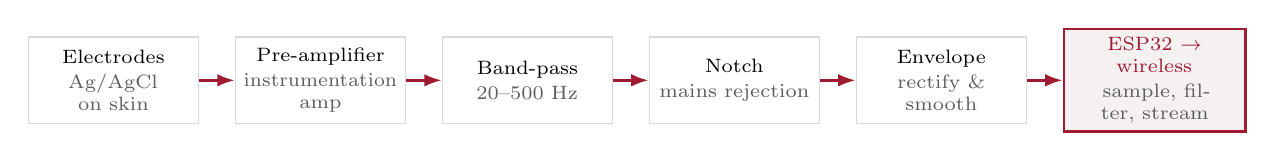
\begin{tikzpicture}[node distance=4mm and 4.5mm]
  \node[bx,text width=1.95cm] (e)  {Electrodes\\[1pt]\textcolor{htilgray}{Ag/AgCl on skin}};
  \node[bx,text width=1.95cm,right=of e] (p)  {Pre-amplifier\\[1pt]\textcolor{htilgray}{instrumentation amp}};
  \node[bx,text width=1.95cm,right=of p] (b)  {Band-pass\\[1pt]\textcolor{htilgray}{20--500 Hz}};
  \node[bx,text width=1.95cm,right=of b] (nf) {Notch\\[1pt]\textcolor{htilgray}{mains rejection}};
  \node[bx,text width=1.95cm,right=of nf] (ev) {Envelope\\[1pt]\textcolor{htilgray}{rectify \& smooth}};
  \node[bxr,text width=2.1cm,right=of ev] (m) {\textcolor{htilred}{ESP32 $\to$ wireless}\\[1pt]\textcolor{htilgray}{sample, filter, stream}};
  \draw[fl] (e) -- (p);
  \draw[fl] (p) -- (b);
  \draw[fl] (b) -- (nf);
  \draw[fl] (nf) -- (ev);
  \draw[fl] (ev) -- (m);
\end{tikzpicture}
\end{center}
\vspace{-2pt}
\noindent{\color{htilrule}\rule{\linewidth}{0.4pt}}\par\vspace{3pt}
\noindent
{\color{htilfaint}\fontsize{7.5}{9}\selectfont\emph{Analog front end --- the stage students wire, filter, and debug}}\hfill
{\color{htilfaint}\fontsize{7.5}{9}\selectfont\emph{Digital --- the stage students program}}\par

\vspace{9pt}\hairline\vspace{4pt}
\eyebrow{Signal sources in the same classroom budget}
\vspace{2pt}

{\fontsize{8.3}{10.2}\selectfont
\begin{tabularx}{\linewidth}{@{}>{\bfseries}p{4.9cm} p{2.1cm} X@{}}
\toprule
Option & Typical cost & Best for \\
\midrule
MioPod --- lab design, ESP32-based & $\approx$\$4 in parts & A station a school can afford to own thirty of; full-station target under \$25 \\
Pre-assembled entry-level EMG module & $\sim$\$10 & Fastest path to a working classroom demo \\
Through-hole soldering EMG kit & $\sim$\$7 & A build-your-own-sensor lab where assembly is the lesson \\
Higher-fidelity EMG module & $\sim$\$31 & Student research projects needing cleaner signal \\
Commercial EMG system & \$200--\$2,000+ & Clinical and research labs --- out of reach at class scale \\
\bottomrule
\end{tabularx}\par}

\vspace{4pt}
{\color{htilgray}\small Ranges reflect the lab's survey of open-source and commercial EMG hardware; per-unit prices fall further at classroom quantity.\par}

\clearpage
% ============================== PAGE 5 ==============================
\eyebrow{Teachers \& Outreach}
\headsm{Building the Teacher Pipeline First}
\standfirst{A tool a teacher cannot troubleshoot is a tool a teacher abandons. Most of the lab's K--12 effort goes into the people who carry the technology into a classroom --- and keep it running.}
\hairline
\vspace{4pt}

\begin{multicols}{2}
Biosignals are noisy. A sensor that worked in a workshop can misbehave on a Monday morning with thirty students, and the difference between a program that spreads and one that stalls is whether a teacher can diagnose the problem. HTIL treats that as a design constraint, not an afterthought: professional development, plain-language materials, and support for the first three lessons matter as much as the software itself.

The lab's teacher-facing work runs through a set of funded programs. An \textbf{NSF RET Site} trains Alabama STEM teachers in sensing technologies, bringing educators into the lab to work on research-grade equipment they then take back to their schools. That site is itself the successor to earlier teacher-training work that has reached on the order of two dozen pre- and in-service teachers, alongside a decade of summer camps and neuro-camps that have put physiological computing in front of roughly 800 K--12 students.

The \textbf{Alabama Power Foundation} supports expansion specifically into West Alabama and the Black Belt --- the rural and historically underserved communities where a low-cost, self-contained station has the most to offer, and where NSF broadening-participation priorities point. The lab's NSF CAREER award takes the same question directly: how do students in rural schools engage with physiological interfaces when the technology comes to them?
\end{multicols}

\vspace{6pt}\hairline\vspace{5pt}
\noindent
\begin{minipage}[t]{0.49\linewidth}
  {\fontsize{10.5}{12}\selectfont\bfseries What teachers get}\par\vspace{2pt}
  \begin{itemize}
    \item A start-up path that does not assume a neuroscience background
    \item Lesson sequences with a clear first, second, and third lesson
    \item Guidance on the failure modes that actually happen in class --- bad contact, motion artifact, mains noise
    \item Hardware students can see into, so a fault is a puzzle rather than a mystery
    \item Curriculum mapped to state standards, so the lesson earns its slot in the year
  \end{itemize}
\end{minipage}%
\hfill
\begin{minipage}[t]{0.47\linewidth}
  {\fontsize{10.5}{12}\selectfont\bfseries Where the work reaches}\par\vspace{2pt}
  {\fontsize{8.3}{10.2}\selectfont
  \begin{tabularx}{\linewidth}{@{}>{\bfseries}p{2.25cm}X@{}}
    Alabama & Pilot classrooms and camps statewide; statewide rollout in discussion with the state education agency \\
    Black Belt & Expansion funded by the Alabama Power Foundation \\
    FL \textperiodcentered\ GA \textperiodcentered\ IL & Partner interest from teacher connections \\
    DMV area & Strategic target for national scale \\
  \end{tabularx}\par}
\end{minipage}

\vspace{8pt}
\begin{tcolorbox}[hbox]
  \boxhead{The un-failable first lesson}
  \vspace{1pt}
  {\small The lab's classroom design assumes the first session must succeed for every student, not just the confident ones. The recommended opener is a mirror, not a challenge: put the sensor on, watch your own signal move, and see how blinking, clenching, or relaxing changes the trace. Nothing to get right, nothing to fail --- but by the end of the lesson every student understands what a biosignal is, from the inside.\par}
\end{tcolorbox}

\statband
  {$\sim$800}{K--12 students reached through camps and classroom programs over roughly a decade}%
  {$\sim$25}{Pre- and in-service teachers trained in sensing technologies through the lab's PD programs}%
  {10+}{Years of classroom research behind the current tools and curriculum}%
  {700+}{Public schools across Alabama --- the reach a statewide rollout would put within range}

\clearpage
% ============================== PAGE 6 ==============================
\eyebrow{Impact \& Next}
\headsm{What's Next for K--12 at HTIL}
\standfirst{The lab's education work is entering a phase where the question shifts from ``does this work in a classroom?'' to ``how does it reach every classroom that wants it?''}
\hairline
\vspace{4pt}

\noindent
\begin{minipage}[t]{0.615\linewidth}
  \begin{multicols}{2}
  Three things are converging. Consumer-grade brain and muscle sensors have dropped below the price point where a school can reasonably buy them. Funding agencies are actively prioritizing broadening participation in computing. And public familiarity with neurotechnology --- for better and worse --- has never been higher, which makes the classroom conversation easier to start and more important to get right.

  HTIL's position is unusual: the research, the software, the hardware, and the competition format all sit in one lab, and all of it has already been in front of students. That makes the next steps concrete rather than speculative --- widening the platforms the software runs on, formalizing the curriculum and teacher certification around it, and turning the Brain Drone Race from an event into a competition circuit that schools can enter the way they enter a robotics league.

  It also brings responsibilities. Recording physiological data from minors raises real privacy and ethics questions, and the lab's approach is to treat those as design requirements from the start --- keeping data handling transparent, minimizing what leaves a student's device, and framing the whole enterprise as \emph{physiological literacy}: learning how your own body works, rather than upgrading it.
  \end{multicols}
\end{minipage}%
\hfill
\begin{minipage}[t]{0.36\linewidth}
  \begin{tcolorbox}[hbox]
    \boxhead{Get involved}
    \vspace{2pt}
    {\fontsize{8.4}{10.5}\selectfont
    {\sffamily\bfseries\color{htilred}\fontsize{7}{8}\selectfont\textls[80]{REQUEST SOFTWARE ACCESS}}\\ htilua.org/neuroblock\\[3pt]
    {\sffamily\bfseries\color{htilred}\fontsize{7}{8}\selectfont\textls[80]{BRING A PILOT TO YOUR SCHOOL}}\\ crawford@cs.ua.edu\\[3pt]
    {\sffamily\bfseries\color{htilred}\fontsize{7}{8}\selectfont\textls[80]{PARTNER ON RESEARCH}}\\ HTIL, Dept.\ of Computer Science\\ The University of Alabama\\[3pt]
    {\sffamily\bfseries\color{htilred}\fontsize{7}{8}\selectfont\textls[80]{PHONE}}\\ (205) 348-6378\par}
  \end{tcolorbox}
  \vspace{6pt}
  \begin{tcolorbox}[obox]
    \boxhead{Lab direction}
    \vspace{1pt}
    {\small HTIL is directed by \textbf{Dr.\ Chris Crawford}, Associate Professor of Computer Science at The University of Alabama. The lab's work spans brain--computer interfaces, human--robot interaction, and physiological computing education.\par}
  \end{tcolorbox}
\end{minipage}

\vspace{8pt}\hairline\vspace{4pt}
\eyebrow{The research behind the classroom}
\vspace{2pt}

{\fontsize{8.3}{10.2}\selectfont
\begin{tabularx}{\linewidth}{@{}>{\bfseries}p{5.6cm} X@{}}
\toprule
Selected funded programs & Focus \\
\midrule
NSF CAREER Award --- \$798K & Engaging rural students with physiological interfaces \\
NSF --- \$1.1M & Elementary physiological computing curriculum \\
NSF RET Site --- \$602K & Training Alabama STEM teachers in sensing technologies \\
NSF (Co-PI) --- \$1.2M & Sensing for data science: web platform for classroom data work \\
NIH (Co-PI) --- \$2.5M & Sensor-based adaptive interventions \\
Alabama Power Foundation --- \$300K & West Alabama / Black Belt educational expansion \\
Intel --- \$300K & Brain--robot interaction \\
\bottomrule
\end{tabularx}\par}

\vspace{8pt}\hairline\vspace{4pt}
\noindent
\begin{minipage}[t]{0.60\linewidth}
  {\color{htilgray}\small This newsletter is a working draft prepared for internal review. Figures, program descriptions, and quotes should be verified against current project documentation before any external distribution.\par}
\end{minipage}%
\hfill
\begin{minipage}[t]{0.37\linewidth}\raggedleft
  {\color{htilgray}\fontsize{7.6}{10}\selectfont The Signal --- K--12 Education in Physiological Computing\\ Human--Technology Interaction Lab \textperiodcentered\ The University of Alabama\\ \textcolor{htilred}{htilua.org}\par}
\end{minipage}

\end{document}
